\documentclass[border=12pt]{standalone}
\def\pgfsysdriver{pgfsys-dvisvgm.def}
\usepackage[dvisvgm]{xcolor}
\usepackage{xeCJK}
\setCJKmainfont{HaranoAjiGothic-Regular.otf}[BoldFont=HaranoAjiGothic-Bold.otf]
\setCJKsansfont{HaranoAjiGothic-Regular.otf}[BoldFont=HaranoAjiGothic-Bold.otf]
\usepackage{amsmath,amssymb,tikz,lmodern}
\usetikzlibrary{arrows.meta,positioning,calc,fit,backgrounds}
\renewcommand{\familydefault}{\sfdefault}
\definecolor{ink}{HTML}{25322F}
\definecolor{green}{HTML}{246657}
\definecolor{tint}{HTML}{EEF4F0}
\definecolor{soft}{HTML}{C6D2CC}
\definecolor{muted}{HTML}{52615B}
\newif\ifJapanese
\newcommand{\Tx}[2]{\ifJapanese #1\else #2\fi}
\newcommand{\Eff}{\overline{\operatorname{Eff}}}
\newcommand{\heading}[3]{{\color{green}\bfseries #1\quad\Tx{#2}{#3}}\\[5pt]}
% A white rectangle makes the complete citation label clickable, including spaces.
\newcommand{\refurl}[2]{\special{dvisvgm:raw <a xlink:href="#1" target="_blank" rel="noopener noreferrer">}{\setlength{\fboxsep}{0pt}\colorbox{white}{\color{green}\underline{\strut #2}}}\special{dvisvgm:raw </a>}}
\tikzset{
 card/.style={draw=soft,fill=white,rounded corners=2pt,align=left,text=ink,font=\fontsize{10.5}{14}\selectfont,inner xsep=12pt,inner ysep=10pt,text width=14.4cm},
 half/.style={card,text width=6.45cm,minimum height=2.05cm},
 result/.style={card,draw=green,fill=tint,line width=.9pt},
 reason/.style={align=left,text=muted,font=\fontsize{9}{12}\selectfont,inner sep=0pt,text width=12.7cm},
 branchreason/.style={reason,text width=5.95cm},
 edge/.style={-{Stealth[length=2.4mm]},draw=green,line width=1pt},
 wire/.style={draw=green,line width=1pt},
}
% Keep the arrow in a dedicated left gutter; explanations never cover it.
\newcommand{\flow}[3]{
 \coordinate (#2-from) at ($(#1.south)+(-6.9,0)$);
 \coordinate (#2-to) at ($(#2.north)+(-6.9,0)$);
 \draw[edge] (#2-from)--(#2-to);
 \node[reason,anchor=west] (#2-reason) at ($(#2-from)!.5!(#2-to)+(.55,0)$) {#3};
}

\newcommand{\Cite}[2]{\refurl{#1}{#2}}

\Japanesetrue
\begin{document}
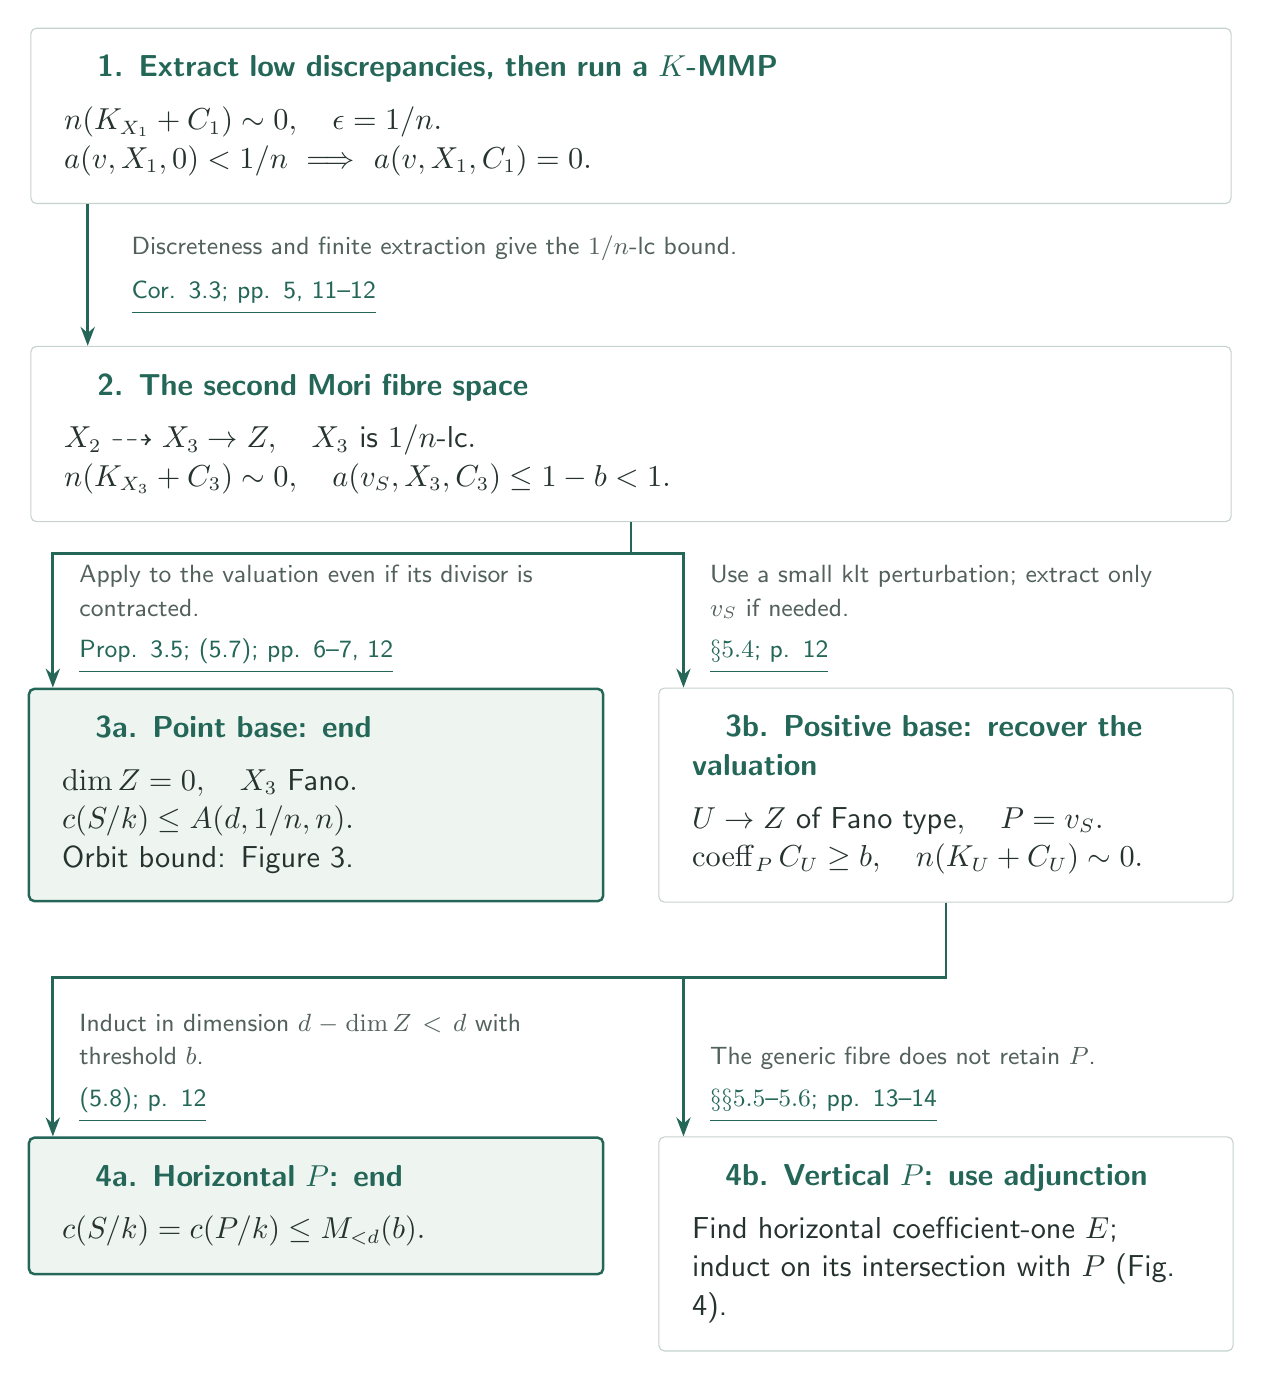
\begin{tikzpicture}
\node[card] (input) {\heading{}{1. 低discrepancyを抽出して $K$-MMP}{1. Extract low discrepancies, then run a $K$-MMP}$n(K_{X_1}+C_1)\sim0,\quad\epsilon=1/n.$\\ $a(v,X_1,0)<1/n\ \Longrightarrow\ a(v,X_1,C_1)=0.$};

\node[card,below=1.8cm of input] (mori) {\heading{}{2. 第2のMoriファイバー空間}{2. The second Mori fibre space}$X_2\dashrightarrow X_3\to Z,\quad X_3\text{ is }1/n\text{-lc}.$\\ $n(K_{X_3}+C_3)\sim0,\quad a(v_S,X_3,C_3)\le1-b<1.$};

\flow{input}{mori}{\Tx{指数の離散性と有限抽出で $1/n$-lc性を確保。}{Discreteness and finite extraction give the $1/n$-lc bound.}\\[4pt]\Cite{https://github.com/openai/math/blob/adc7f1241b42e322a6451854ab7e4b4c146bf78a/preprints/Arithmetic-Stein-degree-bounds-for-log-Calabi-Yau-pairs-September-25-2026/paper.pdf}{Cor. 3.3; pp. 5, 11--12}}
\node[result,text width=6.45cm,below=2.1cm of mori.south,xshift=-4cm] (point) {\heading{}{3a. 点の底：終了}{3a. Point base: end}$\dim Z=0,\quad X_3\text{ Fano}.$\\ $c(S/k)\le A(d,1/n,n).$\\ \Tx{軌道評価は第3図。}{Orbit bound: Figure 3.}};

\node[half,below=2.1cm of mori.south,xshift=4cm] (recover) {\heading{}{3b. 正次元の底：付値を回復}{3b. Positive base: recover the valuation}$U\to Z\text{ of Fano type},\quad P=v_S.$\\ $\operatorname{coeff}_{P}C_U\ge b,\quad n(K_U+C_U)\sim0.$};

\coordinate (point-a) at ($(point.north west)+(.32,0)$);
\draw[edge] (mori.south) -- ++(0,-.4) -| (point-a);
\node[branchreason,anchor=south west] at ($(point.north west)+(.65,.18)$) {\Tx{元の因子が消えていても付値に適用。}{Apply to the valuation even if its divisor is contracted.}\\[3pt]\Cite{https://github.com/openai/math/blob/adc7f1241b42e322a6451854ab7e4b4c146bf78a/preprints/Arithmetic-Stein-degree-bounds-for-log-Calabi-Yau-pairs-September-25-2026/paper.pdf}{Prop. 3.5; (5.7); pp. 6--7, 12}};

\coordinate (recover-a) at ($(recover.north west)+(.32,0)$);
\draw[edge] (mori.south) -- ++(0,-.4) -| (recover-a);
\node[branchreason,anchor=south west] at ($(recover.north west)+(.65,.18)$) {\Tx{小さいklt摂動の下で、必要なら $v_S$ だけ抽出。}{Use a small klt perturbation; extract only $v_S$ if needed.}\\[3pt]\Cite{https://github.com/openai/math/blob/adc7f1241b42e322a6451854ab7e4b4c146bf78a/preprints/Arithmetic-Stein-degree-bounds-for-log-Calabi-Yau-pairs-September-25-2026/paper.pdf}{$\S5.4$; p. 12}};

\node[result,text width=6.45cm,below=7.8cm of mori.south,xshift=-4cm] (horizontal) {\heading{}{4a. $P$ が水平：終了}{4a. Horizontal $P$: end}$c(S/k)=c(P/k)\le M_{<d}(b).$};

\node[half,below=7.8cm of mori.south,xshift=4cm] (vertical) {\heading{}{4b. $P$ が垂直：随伴へ}{4b. Vertical $P$: use adjunction}\Tx{水平係数1成分 $E$ を作り、\\$P$ との交差へ帰納する（第4図）。}{Find horizontal coefficient-one $E$;\\induct on its intersection with $P$ (Fig. 4).}};

\coordinate (horizontal-a) at ($(horizontal.north west)+(.32,0)$);
\draw[edge] (recover.south) -- ++(0,-.95) -| (horizontal-a);
\node[branchreason,anchor=south west] at ($(horizontal.north west)+(.65,.18)$) {\Tx{次元 $d-\dim Z<d$、係数下限 $b$ で帰納。}{Induct in dimension $d-\dim Z<d$ with threshold $b$.}\\[3pt]\Cite{https://github.com/openai/math/blob/adc7f1241b42e322a6451854ab7e4b4c146bf78a/preprints/Arithmetic-Stein-degree-bounds-for-log-Calabi-Yau-pairs-September-25-2026/paper.pdf}{(5.8); p. 12}};

\coordinate (vertical-a) at ($(vertical.north west)+(.32,0)$);
\draw[edge] (recover.south) -- ++(0,-.95) -| (vertical-a);
\node[branchreason,anchor=south west] at ($(vertical.north west)+(.65,.18)$) {\Tx{一般ファイバーには $P$ が残らない。}{The generic fibre does not retain $P$.}\\[3pt]\Cite{https://github.com/openai/math/blob/adc7f1241b42e322a6451854ab7e4b4c146bf78a/preprints/Arithmetic-Stein-degree-bounds-for-log-Calabi-Yau-pairs-September-25-2026/paper.pdf}{$\S\S5.5$--$5.6$; pp. 13--14}};

\end{tikzpicture}
\end{document}
